\documentclass[letterpaper]{article}
\usepackage{amssymb}
\usepackage{fullpage}
\usepackage{changepage}
\usepackage{amsmath}
\usepackage{epsfig,float,alltt}
\usepackage{psfrag,xr}
\usepackage[T1]{fontenc}
\usepackage{url}
\usepackage{pdfpages}
\usepackage{epstopdf}
\usepackage[framed,numbered,autolinebreaks,useliterate]{mcode}

%\includepdfset{pagecommand=\thispagestyle{fancy}}
\author{Fan Bu, Feng Zhou, Yi Yang}
\title{ME 552 Lab 02A Report}

\begin{document}
\date{09/25/2016}
\maketitle

\newcommand{\trace}{\mathrm{trace}}
\newcommand{\real}{\mathbb R}  % real numbers  {I\!\!R}
\newcommand{\nat}{\mathbb N}   % Natural numbers {I\!\!N}
\newcommand{\cp}{\mathbb C}    % complex numbers  {I\!\!\!\!C}
\newcommand{\ds}{\displaystyle}
\newcommand{\mf}[2]{\frac{\ds #1}{\ds #2}}
\newcommand{\spanof}[1]{\textrm{span} \{ #1 \}}
\newcommand{\sol}[0]{\textbf{Solution: }}
\newcommand{\pf}[0]{\textbf{Proof:}}
\newcommand{\rme}[0]{\textrm{e}}
\newcommand{\Null}[1]{\textrm{Null}\{#1\}}
\parindent 0pt
%%%%%%%%%%%%%%%%%%%%%%%%%%%%%%%%%%%%%%%%%%%%%%%%%%%%%%%%%%%%%%%%%%%%%%%%%%%%%%%
% Solution for Question 1 begins here - by Yi Yang
%%%%%%%%%%%%%%%%%%%%%%%%%%%%%%%%%%%%%%%%%%%%%%%%%%%%%%%%%%%%%%%%%%%%%%%%%%%%%%%
\section*{Question 1}
\subsection*{(a)}
Present a block diagram of the closed loop control system, provide all numerical values to the controller and make sure that all details are provided in the figure, the block diagram is provided as below:
\begin{figure}[H]
	\centering
	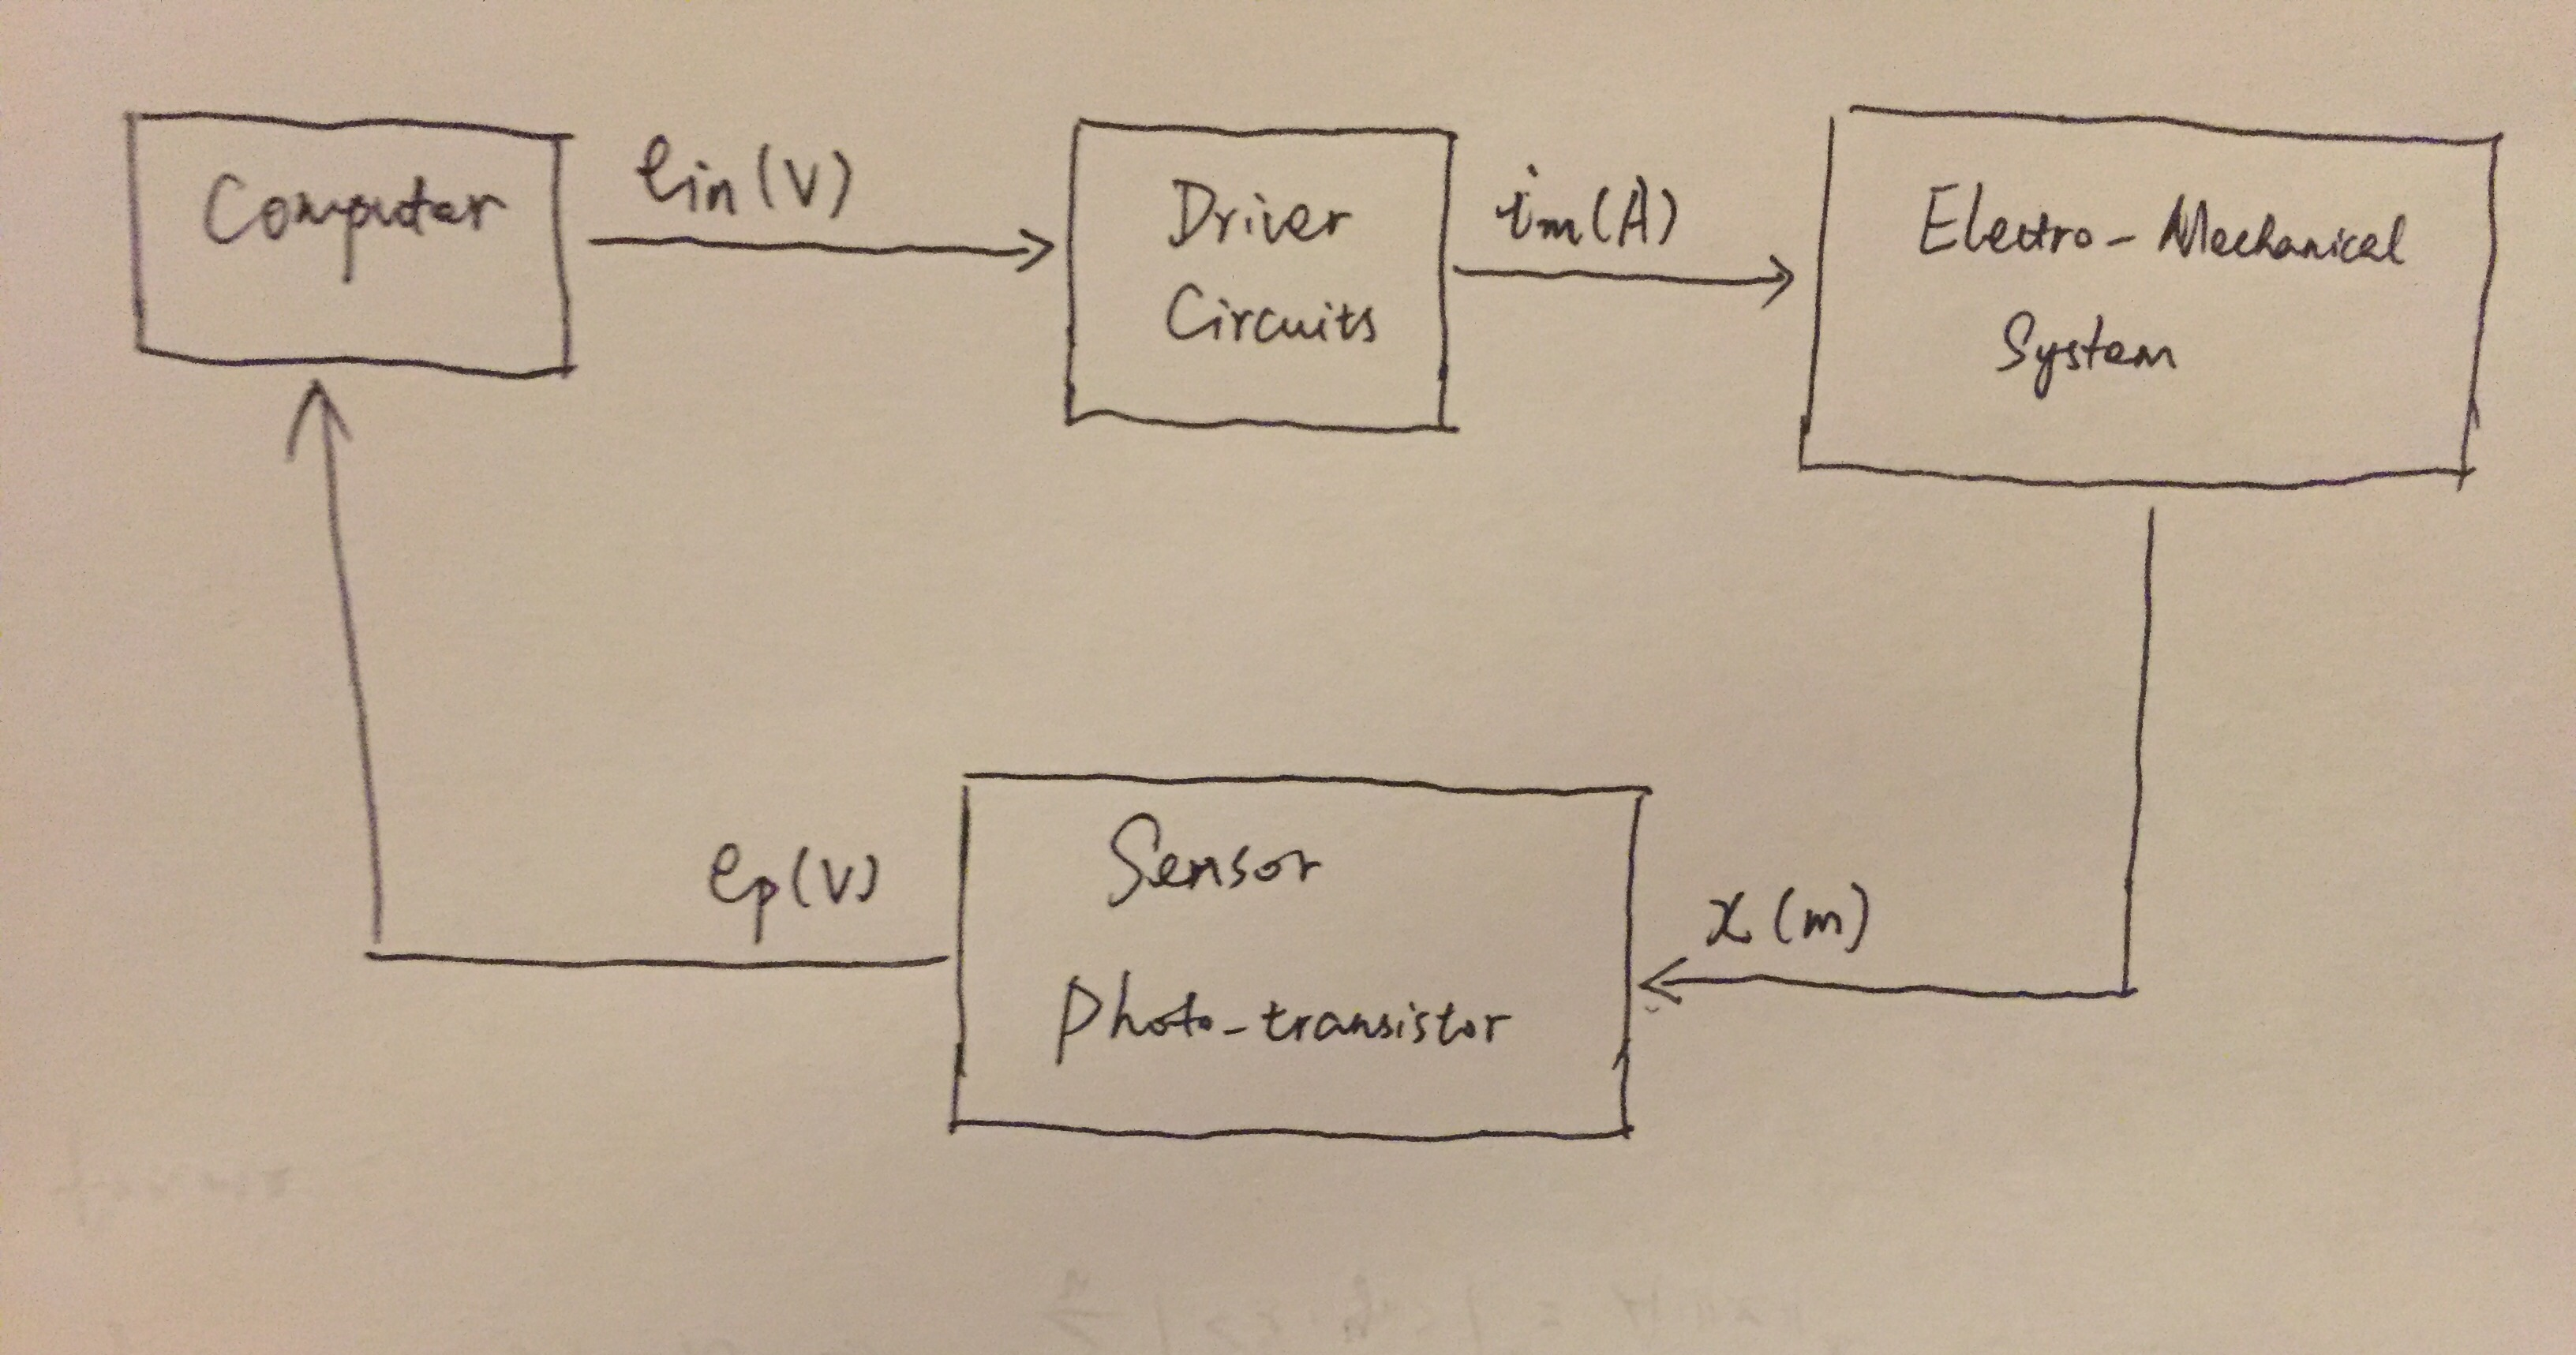
\includegraphics[scale=0.1]{maglev.jpeg}
	\caption{Maglev System Block Diagram}
\end{figure}
It is a brief scheme of maglev system block diagram, we implement a PD controller in Labview and use sisotool in Matlab to tune parameters for controller. First set the desired equilibrium position to be $\bar{x} = 4.19mm$, bias voltage to be $1.85 V$, the open loop system can be:
$$\mf{\hat{X}(s)}{\hat{I}(s)} = \mf{-51}{s^2 - 4685}$$
The next step is to tune PD controller in sisotool. We snapshot the tune results from Matlab, the PD controller is:
$$D(s) = \mf{-2000-5.6s}{1+0.0079s}$$
We need to tune P and D gain to make Labview PD controller match with Matlab PD controller.
\begin{figure}[H]
\centering
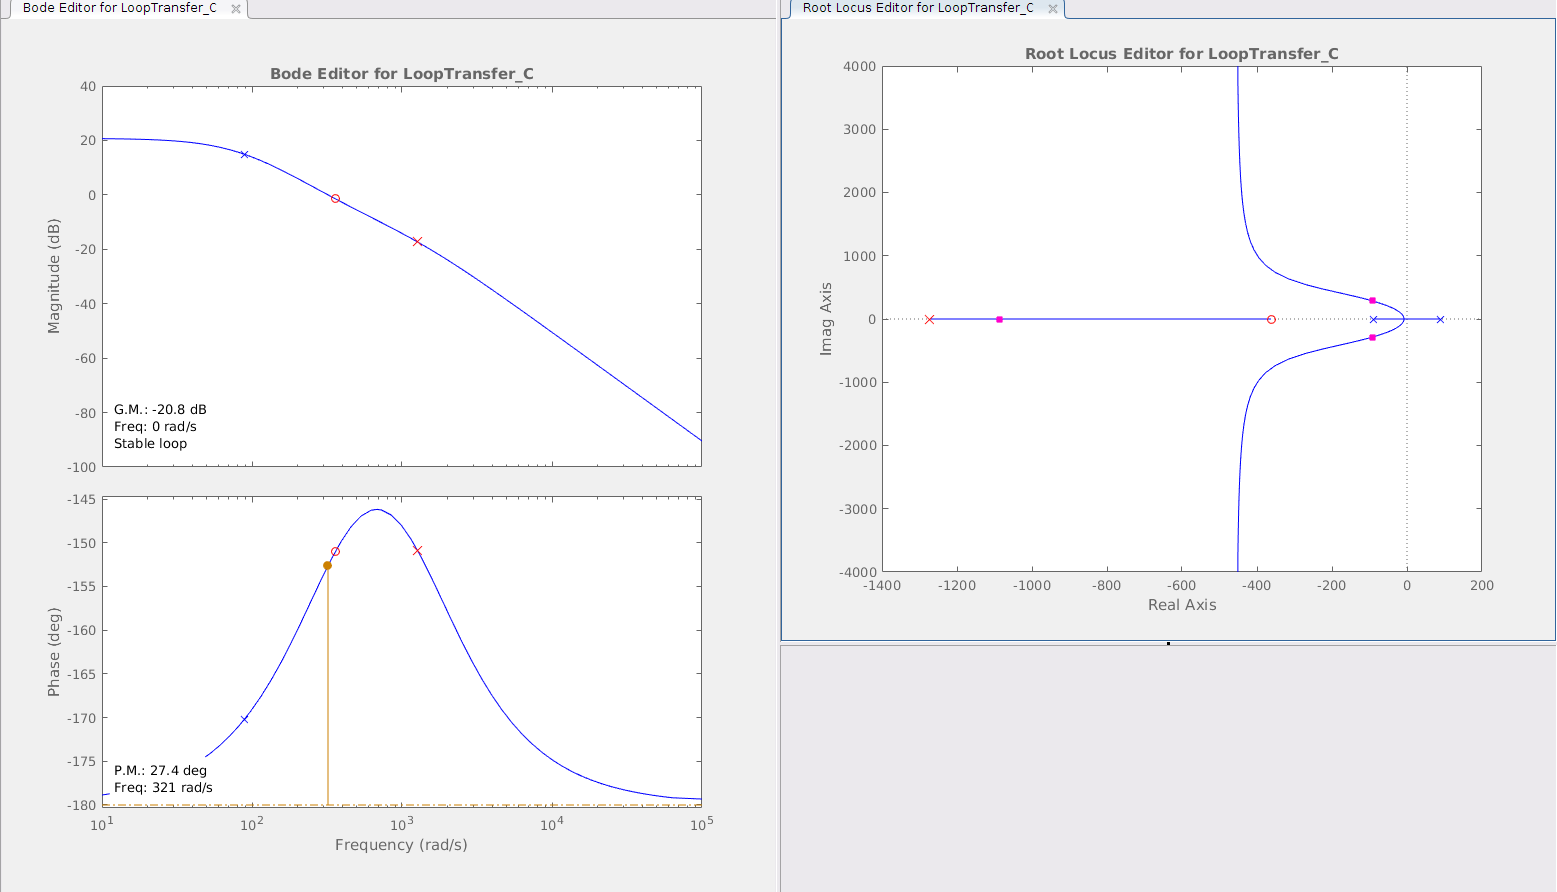
\includegraphics[scale=0.3]{sisotool.png}
\caption{Sisotool Snapshot }
\end{figure}
\subsection*{(b)}
Present the mathematical and physical meaning of bias voltage, the bias voltage performs two functions in the circuits:
\begin{itemize}
	\item Since the control loop is used for controlling the position variation of the floating ball, denoted by $\hat{x}$, and we want the control be performed around a point of interest, denoted by $x_\circ$. Hence, we need to apply a bias voltage to the driver circuits to make our magnet attract the steel to stay at the position of our interest at the steady state without error.
	\item The PD controller can only speed up the rate of convergence to the steady state, but it can not counteract the steady state error when there is a tiny disturbance to the ball. However, the steady error is constant, we could use an offset voltage or integral controller to compensate the steady state error.
	
\end{itemize}
\subsection*{(c)}
Justify why a buffer circuit will be used for the output of a sensor set-up:\\
The photo-transistor will generate a current with intensity proportional to the light it receives from emitter. However, we could only input signal to the DAQ system in the form of voltage. Hence, we need a resistor to transform the current into voltage and calibrate the value of resistor to make the range of input voltage from $0 V$ to $10 V$. Also we need add a buffer circuit behind sensor circuit to avoid loading effects. Though the input resistance of DAQ circuits is very large, we can still use the buffer circuits in case of the sensor circuits are directly connected to some components with low input resistance.
\subsection*{(d)}
Determine the minimum value of the resistance that can be used in the emitter circuit and describe the significance of the resistor, the circuit for the emitter circuit is shown below:
\begin{figure}[H]
	\centering
	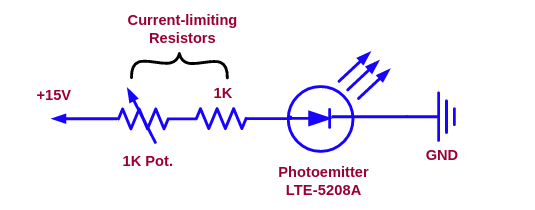
\includegraphics[scale=0.8]{emitter_circuit.png}
	\caption{Emitter Circuit}
	\label{fig:emiter_circuit}
\end{figure}
Check the data sheet of Photoemitter $LTE\-5208A$, we get the following data: the maximum of forward voltage for transistor is $1.6 V$, the maximum continuous forward current is $100mA$, hence we can use these values to approximate the minimum value for our potentiometer.
$$V_{CL} = 15V - 1.6V = 13.4V$$
$$R_{CL} = \mf{V_{CL}}{100\times10^{-3}A} = 134\Omega$$
The minimum value for the current limit resistance is $134\Omega$. The lower resistance will result in a higher current for our circuit, the photo-emitter will have higher power dissipation which will make the light much brighter, thus the sensing performance will be better. However, we need to calibrate the resistance value of emitter circuit and photo-transistor circuit to make sure the output voltage range from $0 V$ to $10 V$.
\subsection*{(e)}
First, we need to calculate the maximum current that the magnetic coil could ever see, the voltage current driver circuit is shown as below:
\begin{figure}[H]
	\centering
	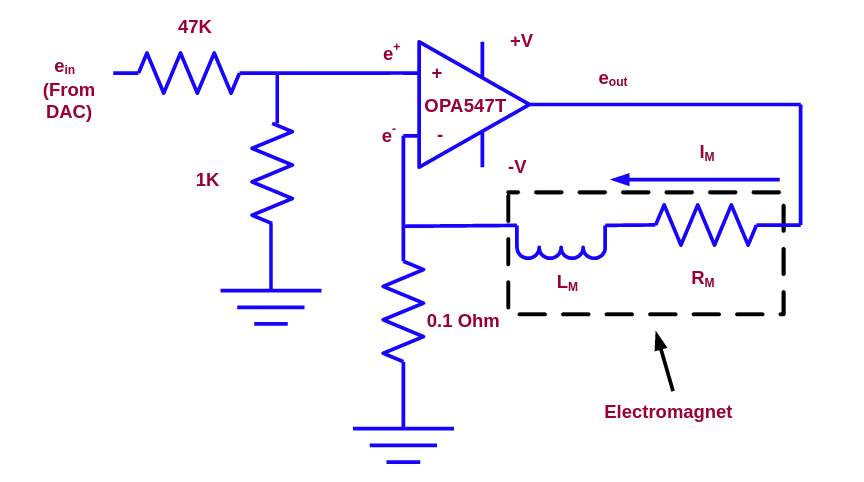
\includegraphics[scale=0.4]{current_driver_circuit.png}
	\caption{Voltage Current Circuit}
	\label{fig:vcc}
\end{figure}
As for OPA$547$T Op-Amp, we can set $R_{CL}$ to limit the current that passes electromagnet coils. We will calculate the the maximum current with following circuit failures:
\begin{itemize}
	\item $R_{CL}$ is shorted out of our circuit, the maximum current can be $750mA$.
	\item $R_{CL}$ is set to be $15K\Omega$, the maximum current can be $$\mf{4.75V\times 5000}{31.6K\Omega + 15K\Omega} = 509.7mA$$
\end{itemize}
The circuit is operating in the normal state if we set correct values to $R_{CL}$ to limit the current passing through electromagnet. However, if our electromagnet is directly connected to the two poles of power supply, the internal resistance for electromagnet circuit is $35\Omega$ when it is open, thereby we can get the power dissipation in this case:
$$P = \mf{(30V)^2}{35\Omega} = 25.714W$$
$$I = \mf{30V}{35\Omega} = 857mA$$
The coil inside electromagnet will absolutely be melt. In order to avoid such damage to the coil, we recommend adding a fuse connecting in series with the coil and the limit current to the fuse can be a little bit higher than the coil current rating value.
\subsection*{(f)}
The saturation limits on the analog out $2.4V$, the voltage $e_{in}$ input to Op-Amp can be ranged from $0$ to $2.4V$. The current limit to our circuit is $509.7mA$. We can use this value to get:
$$e_{in} = \mf{R_s(R_1 + R_2)}{R_2}I_m = \mf{0.1\times (44200 + 984)}{984}\times 0.5097 = 2.446V$$
We set analog voltage to be positive in order to avoid non-linear behavior of the electromagnet, since the negative voltage will attract the ball in this non-linear system which is deviated from our expectation to make ball away from magnet when the negative voltage is applied.
\subsection*{(g)}
No, the polarity of electromagnet does not matter in the current driver circuits, since either pole of the magnet could attract the ball and the ball are assumed not to be magnetized permanently when it appears in the magnetic field generated by electromagnet.

\hspace*{2em}
\section*{Appendix}
\begin{figure}[H]
	\centering
	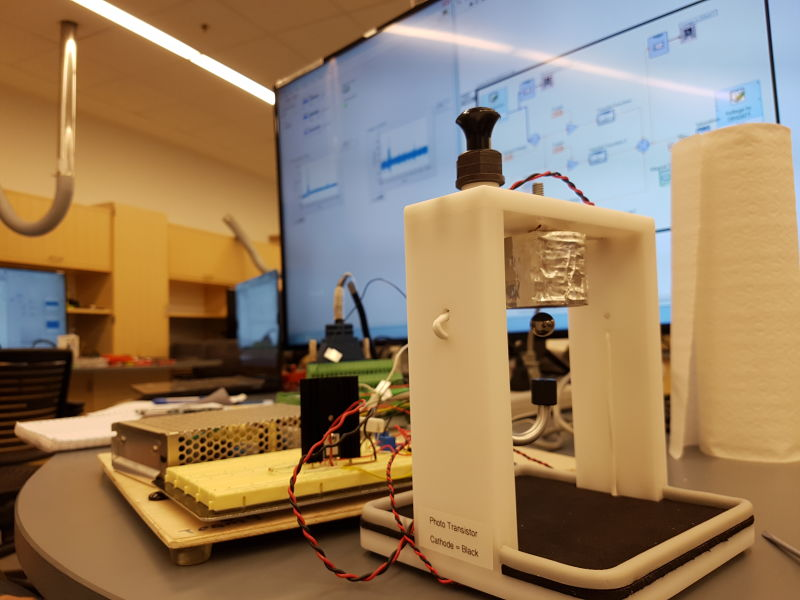
\includegraphics[scale=0.4]{physnapshot.jpeg}
\end{figure}
\end{document}